\documentclass[a4paper,twoside]{article}
\usepackage[utf8]{inputenc}
\usepackage{url}
\usepackage{color}
\usepackage{charter}
\usepackage{caption}
\usepackage{parskip}
\usepackage{graphicx}
\usepackage[margin=1in]{geometry}

%
\newcommand{\shortstandard}{ISO/IEC~18004}
\newcommand{\standard}{\shortstandard:2024(en)}
\newcommand{\quotestandard}[1]{\textcolor{blue}{\textit{#1}}}
\newcommand{\ddd}{\dots}
\newcommand{\change}[1]{\underline{\textbf{#1}}}
\newcommand{\hex}[1]{#1(hex)}

\newcommand{\best}[1]{\underline{#1}}
\newcommand{\good}[1]{\textcolor{green}{#1}}
\newcommand{\bad}[1]{\textcolor{red}{#1}}
%
%
%
\captionsetup{margin=10pt,font={small,it}} % Options: tiny, scriptsize, footnotesize, small, normalsize, etc.
%
%
%
\title{Suggested improvements to \standard}
\author{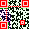
\includegraphics[width=0.2\textwidth]{images/email.png} \\ \\ Sidney~Cadot~\url{<sidney.cadot@gmail.com>}} 

\date{Version 0.1 --- May~2025}
%
%
%
\begin{document}
%
%
\maketitle
%
%
\section{Introduction}

The \standard{} standard describes the encoding and decoding of QR code symbols. With this standard in hand,
I recently implemented a QR code encoder library\footnote{The encoder I implemented can be found on Github:
\url{https://github.com/sidneycadot/qrcodes}.}, mostly to satisfy my curiosity about how QR codes work.

Not surprisingly, a close reading of the standard was necessary to achieve a working encoder. With the benefit
of reading with a 'fresh pair of eyes', several small mistakes were found in the standard text that are easily
fixable. In addition, it was found that a few sections could be improved in terms of understandability. All
these potential improvements are collected in the document that you are currently reading.

My hope is that the standard committee will consider the suggested improvements in order to improve the
quality of the \shortstandard{} standard, and that at least some of the items listed will be addressed in
the next edition.

Most notably, the rather hard to understand description of the data masking pattern scoring algorithm in
Section~7.8.3.1, and the related fact that some of the concrete QR codes shown in the standard appear to
select a non-optimal data masking pattern, leaves room for improvement. This is discussed in
Section~\ref{sec:dmp-scoring}, below.

\section{Suggested improvements}

Below is a list of suggested improvements to the standard. All section and page references are to the most recent (fourth)
edition of the standard, i.e., \standard. Quotes from the standard are shown in \textcolor{blue}{blue}.

\subsection{\standard, Introduction (page vii)}

In the third clause of the enumeration, it is unclear what the sentence fragment below means; it appears to be non-grammatical:

\begin{quote}
\quotestandard{\ddd the option for specifying alternative character is set to the default.}
\end{quote}

It is suggested to reword this for clarity.

\subsection{\standard, Introduction (page vii)}

In the fourth clause of the enumeration, a word appears to be missing.

\begin{quote}
\quotestandard{\ddd which enables small to moderate amount of data to be represented \ddd}
\end{quote}

It is suggested to change this to:

\begin{quote}
\quotestandard{\ddd which enables \change{a} small to moderate amount of data to be represented \ddd}
\end{quote}

\subsection{\standard, Section 5.1, clause b.3 (page 4)}

The default character set for byte data in the absence of an explicit ECI designator is defined here as ISO/IEC~8859-1.

It would be useful to explicitly indicate that in the 2000 edition of the standard, the default encoding was JIS-8,
and that this was changed to ISO/IEC 8859-1 in the 2006 edition of the standard.

Furthermore, it may be useful to mention that, in contradiction to the standard, many modern QR code decoders (e.g. those
implemented on mobile phones) use UTF-8 as the default encoding instead.

\subsection{\standard, Section 5.1, clause f (page 5)}

It is not made clear what these percentages mean, i.e., what the precise guarantee is for any of the four levels of
error correction in terms of error correction capabilities.

As stated, the most natural interpretation of the percentages would be that they indicate that if \emph{any} x\% of the
modules in the entire QR code are damaged (inverted), the QR code would still be readable. However, this is not the
case, as the percentage indicates the fraction of errors that can be dealt with \emph{per block code word} rather than for
the entire QR code, and on the GF(256) symbol level rather than on the bit/module level.

An unlucky set of module-level errors can, in fact, damage the QR code beyond repair with \emph{far less} than the stated
percentages of module-level errors.

It would be helpful if the precise meaning of the percentages given is made clear, as well as what they mean in practical
terms.

\subsection{\standard, Section 5.2, Figure 1 (page 6)}
\label{sec:dmp-changed-1}

The QR code symbol used here as an example uses data masking pattern~6, whereas in earlier editions of the standard
(2000, 2006, 2015), this same example used data masking pattern~5.
These two alternative code symbols are shown in Figure~\ref{fig:dmp-changed-1}).

It would be useful to explicitly acknowledge this change, and explain which one is the correct choice;
see also Sections~\ref{sec:dmp-scoring} and \ref{sec:dmp-changed-2}.

\begin{figure}[h!]
\centering
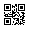
\includegraphics[width=0.4\textwidth]{images/qrcode_iso18004_2000_2006_2015_QRCodeSymbol_1Mp5.png}

\includegraphics[width=0.4\textwidth]{images/qrcode_iso18004_2024_QRCodeSymbol_1Mp6.png}
\caption{The text ``QR Code Symbol'' represented as a 1-M QR code using two different data masking patterns.
         The left version, as found in the 2000, 2006, and 2015 editions of the standard, uses data masking pattern~5.
         The right version, as found in the 2024 edition of the standard, uses data masking pattern~6.}
\label{fig:dmp-changed-1}
\end{figure}

\subsection{\standard, Section 5.2, Figure 1, caption (page 6)}

The caption claims the QR code example encodes the text ``QR code Symbol''.

In fact, the QR code example encodes the text ``QR Code Symbol'', with the word `Code' capitalized.

In earlier editions of the standard (2006, 2015) the caption was correct. This change should be reverted.

\subsection{\standard, Section 7.3.1 (page 18)}

It is unclear what this section is saying, precisely.

\subsection{\standard, Section 7.3.6 (page 18)}

It is unclear what this section is saying, precisely.

\subsection{\standard, Section 7.4.3.2 (page 22)}

The ECI designator example given is incorrect.

In ISO/IEC~8859-7, the five Greek letters A, B, $\Gamma$, $\Delta$, and E are encoded as byte values \hex{C1} to \hex{C5}.
The example shown in this section erroneously encodes them as byte values \hex{A1} to \hex{A5}.

This mistake is also present in the 2000, 2006, and 2015 editions of the standard.

It would also be useful if an example QR code symbol that contains the encoded data is included in the standard (Figure~\ref{fig:greek-encoding}).

\begin{figure}[h]
\centering

\includegraphics[width=0.4\textwidth]{images/qrcode_iso18004_2024_QRCodeSymbol_1Mp6.png}
\caption{The text ``AB$\mathit{\Gamma\Delta}$E'' represented as a 1-H QR code using data masking pattern 6.
         The five bytes values \hex{C1} to \hex{C5} are preceded by an ECI designator that changes the character
         interpretation to the value 000009, indicating that the bytes that follow should be interpreted using
         the ISO/IEC~8859-7 byte-to-character mapping.}
\label{fig:greek-encoding}
\end{figure}

\subsection{\standard, Section 7.4.6, Note 3, 4 (page 26)}

These two notes indicate the differences between Table~6 and ISO/IEC~8859-1, especially in
regard to the interpretation of  the lower 32 byte values.

However, Section~5.1, clause b.3 indicates that the default encoding of bytes blocks
(in absence of a preceding ECI designator) is ISO/IEC~8859-1, which leaves those 32 bytes
undefined.

These statements are in contradiction. Either the default encoding is actually ISO/IEC~8859-1
(with the first 32 byte values undefined) or it is the similar-but-different encoding given
in Table~6, where an interpretation is assigned to the first 32 byte values.

The standard should make an unequivocal choice.

\subsection{\standard, Section 7.4.11 (page 29)}

This text can be improved for readability.

\subsubsection*{First suggestion}

\begin{quote}
\quotestandard{\ddd shall be connected in order \ddd}
\end{quote}

can be changed to:

\begin{quote}
\quotestandard{\ddd shall be \change{concatenated} in order \ddd}
\end{quote}

\subsubsection*{Second suggestion}

\begin{quote}
\quotestandard{In certain versions of symbol \ddd}
\end{quote}

can be changed to:

\begin{quote}
\quotestandard{In certain \change{QR code symbol versions} \ddd}
\end{quote}

\subsection{\standard, Section 7.5.1 (page 33)}

\begin{quote}
\quotestandard{Since QR code is a matrix symbology, a defect converting a module from dark to light or vice versa
will result in the affected symbol character misdecoding as an apparently valid but different codeword.}
\end{quote}

This statement, in particular the part before the comma, does not make sense. The fact that module
inversion will lead to a symbol character misdecoding is true, but this is not `because QR code is a
matrix symbology'.

Deleting the part before the comma improves the clarity of the statement:

\begin{quote}
\quotestandard{\change{A} defect converting a module from dark to light or vice versa will result in the affected symbol
character misdecoding as an apparently valid but different codeword.}
\end{quote}

\subsection{\standard, Section 7.5.1 (page 33, 34)}

The explanation of the $p$ value is overly complicated. Consider rewriting it for clarity.

\subsection{\standard, Section 7.5.1, Table 9 (pages 34 to 40)}

The last two columns of the table are confusing, as each version's entry can have more than the expected
four rows specifying the code block parameters used for each of the four error levels (L, Q, M, H). The
fact that a single specification can span multiple lines, to reflect the fact that a specific
version / error correction level combination can use more than one block code, is not a-priori clear.

Consider adding horizontal separator lines in the last two columns, to show
which code lines correspond to which of the four error correction levels.

Note: the table used to be formatted like that in the corresponding tables in the 2000
and 2006 editions of the standard. The presentation of the same information in those two
editions of the standard is much clearer because of that.

\subsection{\standard, Section 7.8.3.1 (pages 49, 50)}
\label{sec:dmp-scoring}

This section is quite unclear; it would be advisable to re-write it. it is very
hard to ascertain the intended score calculation from this description alone. 

One of the more confusing sentences in this section is this:

\begin{quote}
\quotestandard{\ddd the variables N1 to N4 represent weighted penalty scores for the undesirable features \ddd}
\end{quote}

However, N1 to N4 are not variables, but \emph{constants}; and they don't represent weighted penalty
scores; rather, they are merely constants used in the calculation of the four terms that make up
the final penalty score for a given symbol.

\subsubsection*{Inconsistency between the scoring algorithm and the data masking pattern choices in the example QR codes found in \standard}

More importantly, the score calculation described in this section does not lead to the data masking
pattern choices made for the seven QR code symbol examples given in the standard itself (Figure~1,
Figure~29 with five examples, and Figure~I.4).

Table~\ref{tab:dmp-selections} shows the scores calculated according to the scoring method described, for each of the seven QR codes
found in the standard, and for each of the eight data masking pattern choices. Also listed is the optimal data mask
pattern choice (with the  lowest score) and the data mask pattern actually used in the QR code symbol shown in the standard.

These two data mask pattern choices should match, but for four out of seven cases, they do not.

\begin{table}[h!]
\centering
\tiny
\begin{tabular}{|c|c|c|c|c|c|}
\hline
QR code example & Description & Symbol & Pattern scores P0 to P7 (best score underlined) & Optimal pattern & Pattern used in standard \\
\hline
Figure 1              & ``QR Code Symbol''                       & 1-M & 1219,1195,1189,1182,1142,\best{1107},1116,1198 & Pattern 5 & \bad{Pattern 6}  \\
Figure 29, top        & Structured Append Mode example, combined & 4-M & 1672,1684,1568,\best{1402},1416,1690,1598,1624 & Pattern 3 & \bad{Pattern 4}  \\
Figure 29, second row & Structured Append Mode example, 1 of 4   & 1-M & \best{1097},1146,1208,1174,1136,1164,1184,1128 & Pattern 0 & \good{Pattern 0} \\
Figure 29, second row & Structured Append Mode example, 2 of 4   & 1-M & \best{1095},1192,1203,1167,1133,1178,1171,1103 & Pattern 0 & \bad{Pattern 7}  \\
Figure 29, second row & Structured Append Mode example, 3 of 4   & 1-M & 1119,1125,1191,1134,1196,1137,1123,\best{1090} & Pattern 7 & \good{Pattern 7} \\
Figure 29, second row & Structured Append Mode example, 4 of 4   & 1-M & 1245,1173,1207,\best{1128},1148,1155,1172,1136 & Pattern 3 & \good{Pattern 3} \\
Figure I.4            & ``01234567''                             & 1-M & 1153,1250,1160,\best{1128},1214,1243,1153,1133 & Pattern 3 & \bad{Pattern 2} \\
\hline
\end{tabular}
\caption{Overview of QR codes found in \standard}
\label{tab:dmp-selections}
\end{table}

The clarity of this section could be greatly improved if one or two worked-out examples were added that show the four score
contribution terms and final scores for each of the eight data masking patterns. For example, for the QR code example discussed
in Annex~I, a table such as Table~\ref{tab:dmp-selection-annex-example} lists the four score terms and the total score for each
data masking pattern choice:

\begin{table}[h!]
\centering
\tiny
\begin{tabular}{|c|c|c|c|c|c|}
\hline
Data masking pattern & First score term & Second score term & Third score term & Fourth score term & Total score (best score underlined) \\
\hline
Pattern 0            & 182              & 171               & 800              &  0                & 1153        \\
Pattern 1            & 216              & 234               & 800              &  0                & 1250        \\
Pattern 2            & 235              & 195               & 720              & 10                & 1160        \\
Pattern 3            & 216              & 192               & 720              &  0                & \best{1128} \\
Pattern 4            & 217              & 237               & 760              &  0                & 1214        \\
Pattern 5            & 245              & 220               & 760              & 10                & 1243        \\
Pattern 6            & 207              & 186               & 760              &  0                & 1153        \\
Pattern 7            & 203              & 210               & 720              &  0                & 1133        \\
\hline
\end{tabular}
\caption{Partial and total scores for the QR code discussed in Annex~I}
\label{tab:dmp-selection-annex-example}
\end{table}

\subsubsection*{Missing tie-breaker rule}

A tie-breaker rule should be defined in case two data masking patterns yield an identical score.

This would ensure that, for each QR code, there is a fully deterministic and unambiguous way of selecting the
correct data masking pattern.

\subsubsection*{Specify behavior of decoders when encountering QR codes with sub-optimal data masking pattern}

It is suggested that a statement be added that decoders \emph{should} accept QR codes with a suboptimal data masking
pattern choice.

\subsubsection*{Two further remarks on the score algorithm}

(1) According to the scoring procedure, the scores are determined with the version and format information areas
cleared (light modules). This is an unfortunate and suboptimal choice for which there seems to be no good reason.
It would be better if the standard mandated that both the version and format information were fully filled in when 
scoring the data masking patterns, taking into account that the format version information changes when assessing
the eight data masking patterns in turn.

(2) The fourth term in the scoring algorithm penalizes an imbalance between dark and light
squares in the QR code; but it does so by binning the percentual deviations in `classes' of
deviation away from the ideal 50\% score:

\begin{verbatim}
score_contribution =
    10 * floor(abs(dark_count / (dark_count + light_count) * 100 - 50) / 5)
\end{verbatim}

The reason for applying this discretization is unclear. A more obvious scoring calculation for the
dark/light imbalance would omit the discretization but follow the same linear penalty relation,
at two penalty points per percent of deviation:

\begin{verbatim}
score_contribution_alternative =
    floor(2 * abs(dark_count / (dark_count + light_count) * 100 - 50))
\end{verbatim}

\subsection{\standard, Annex A (page 69)}

The definition of the generator polynomials is not correct:

\begin{quote}
\quotestandard{Each generator polynomial is the product of first degree polynomials: $x - 2^0$, $x - 2^1$, \dots, $x - 2^{n-1}$,
where n is the degree of the generator polynomial.}
\end{quote}

This mixes up the primitive root of GF(256), $\alpha$, with its byte representation, the value 2.

The correct statement is:

\begin{quote}
\quotestandard{Each generator polynomial is the product of first degree polynomials: \change{$x - \alpha^0$}, \change{$x - \alpha^1$}, \dots, \change{$x - \alpha^{n-1}$},
where n is the degree of the generator polynomial.}
\end{quote}

\subsection{\standard, Annex E, Table E.1 (pages 78, 79)}

The description of the alignment pattern position algorithm says:

\begin{quote}
\quotestandard{They are spaced as evenly as possible between the timing pattern and the opposite side of the symbol, any uneven
spacing being accommodated between the timing pattern and the first alignment pattern in the symbol interior.}
\end{quote}

Unfortunately, this doesn't provide enough information on how this accommodation is achieved; it still leaves multiple
possible solutions for each QR code version where the alignment patterns cannot be distributed evenly.

An explanation  of the choice made in those cases would be welcome. Specifically, this concerns the sixteen QR code versions
15, 16, 18, 19, 22, 24, 26, 28, 30, 31, 32, 33, 36, 37, 39, and 40.

\subsection{\standard, Annex I.2.6 (page 90)}
\label{sec:dmp-changed-2}

This subsection contains an incorrect statement:

\begin{quote}
\quotestandard{\ddd the data masking pattern is 011.}
\end{quote}

This should be changed to:

\begin{quote}
\quotestandard{\ddd the data masking pattern is \change{010}.}
\end{quote}

This makes this subsection internally consistent, as the explanation describes that data masking pattern 2 is selected.

It seems that this mistake stems from the 2000 edition of the standard, where the same example was worked out;
except back then, data masking pattern~3 was chosen instead of data masking pattern~2.
These two alternative code symbols are shown in Figure~\ref{fig:dmp-changed-2}).

When updating this section to reflect that change for the 2006 edition, it appears that this particular reference
to data masking pattern 011 was left by accident, and this wasn't corrected in the 2015 and 2024 editions.

\begin{figure}[h!]
\centering

\includegraphics[width=0.4\textwidth]{images/qrcode_iso18004_2000_AnnexG_1Mp3.png}

\includegraphics[width=0.4\textwidth]{images/qrcode_iso18004_2006_2015_2024_AnnexI_1Mp2.png}
\caption{The text ``01234567'' represented as a 1-M QR code using two different data masking patterns.
         The left version, as found in the 2000 edition of the standard, uses data masking pattern 3.
         The right version, as found in the 2006, 2015, and 2024 editions of the standard, uses data masking pattern 2.}
\label{fig:dmp-changed-2}
\end{figure}

It would be useful to explicitly acknowledge this change, and explain which one is the correct choice.

See also Sections~\ref{sec:dmp-changed-1} and \ref{sec:dmp-scoring}.

\subsection{General recommendations}

Once the issues with the data masking pattern scoring are fixed, it would be useful to include more concrete examples
of QR code symbols in the standard, perhaps as an Annex. These could serve as a `gold standard' for implementers of both
encoders and decoders.

For some of the more esoteric parts of the standard (in particular, the codes used for the format information and version areas,
the Reed-Solomon codes used for the information area, and the data masking pattern scoring) it would be very helpful if pseudocode
(or even code in a mainstream programming language, like Python) would be provided, perhaps as an Annex.

\end{document}
